\chapter{Analýza a~návrh řešení}\label{kap:analyza}
% Analýza a~návrh implementace (včetně diskuse různých alternativ a~volby implementačního prostředí).
% 
% Tady bude všechno týkající se návrhu:
% \begin{itemize}
%  \item porty pro PC
%  \item telnet - problemy s klientem ?
%  \item vlakna pro klienty
%  \item asi nejaky obrazky možná i naskenovaný čmárák
%  \item zjišťování, jak funguje Cisco
%  \item UML - tridni diagram
%  \item UML - pruchod parserem
%  \item ..
% \end{itemize}
Jádro aplikace bylo vytvářeno ve spolupráci s kolegou, tudíž následující řádky týkající se architektury systému se mohou v nějaké podobě objevit i v jeho práci. Práce se úmyslně nezabývá striktně mojí vlastní \uv{Cisco částí}, protože tento systém tvoří jeden celek, který je ovlivněn jeho podsystémy. 

V této kapitole je popsáno především společné jádro. Návrh a implementace Cisco části je v kapitole Realizace \ref{realizace}.

%------------------------------------------------------------------------------

\section{Architektura}
Celá aplikace je rozdělena na dvě vrstvy - síťová a aplikační. Síťová vrstva je více popsána v sekci \ref{klien_server}. Aplikační vrstvu tvoří de facto zbytek systému (směrování, překlad adres, parsery příkazů, ..).

%------------------------------------------------------------------------------

\subsection{Počátek prací}
Když jsem dostal ústní zadání této práce, tak jsem hned začal přemýšlet, jak navrhnout celou aplikaci. Zadání ale nebylo specifikováno přesně se všemi potřebnými detaily, takže jsem měl \uv{volnou} ruku co se návrhu týče. Po konzultaci s kolegou vzniklo několik variant, na obrázku \ref{fig:navrh} je jedna z nich. Tato varianta počítala s tím, že počítač bude připojen do reálné sítě, ale byla zavržena po dohodě s vedoucím práce kvůli složitosti a náročnosti takového systému. 

\begin{figure}[h]
\begin{center}
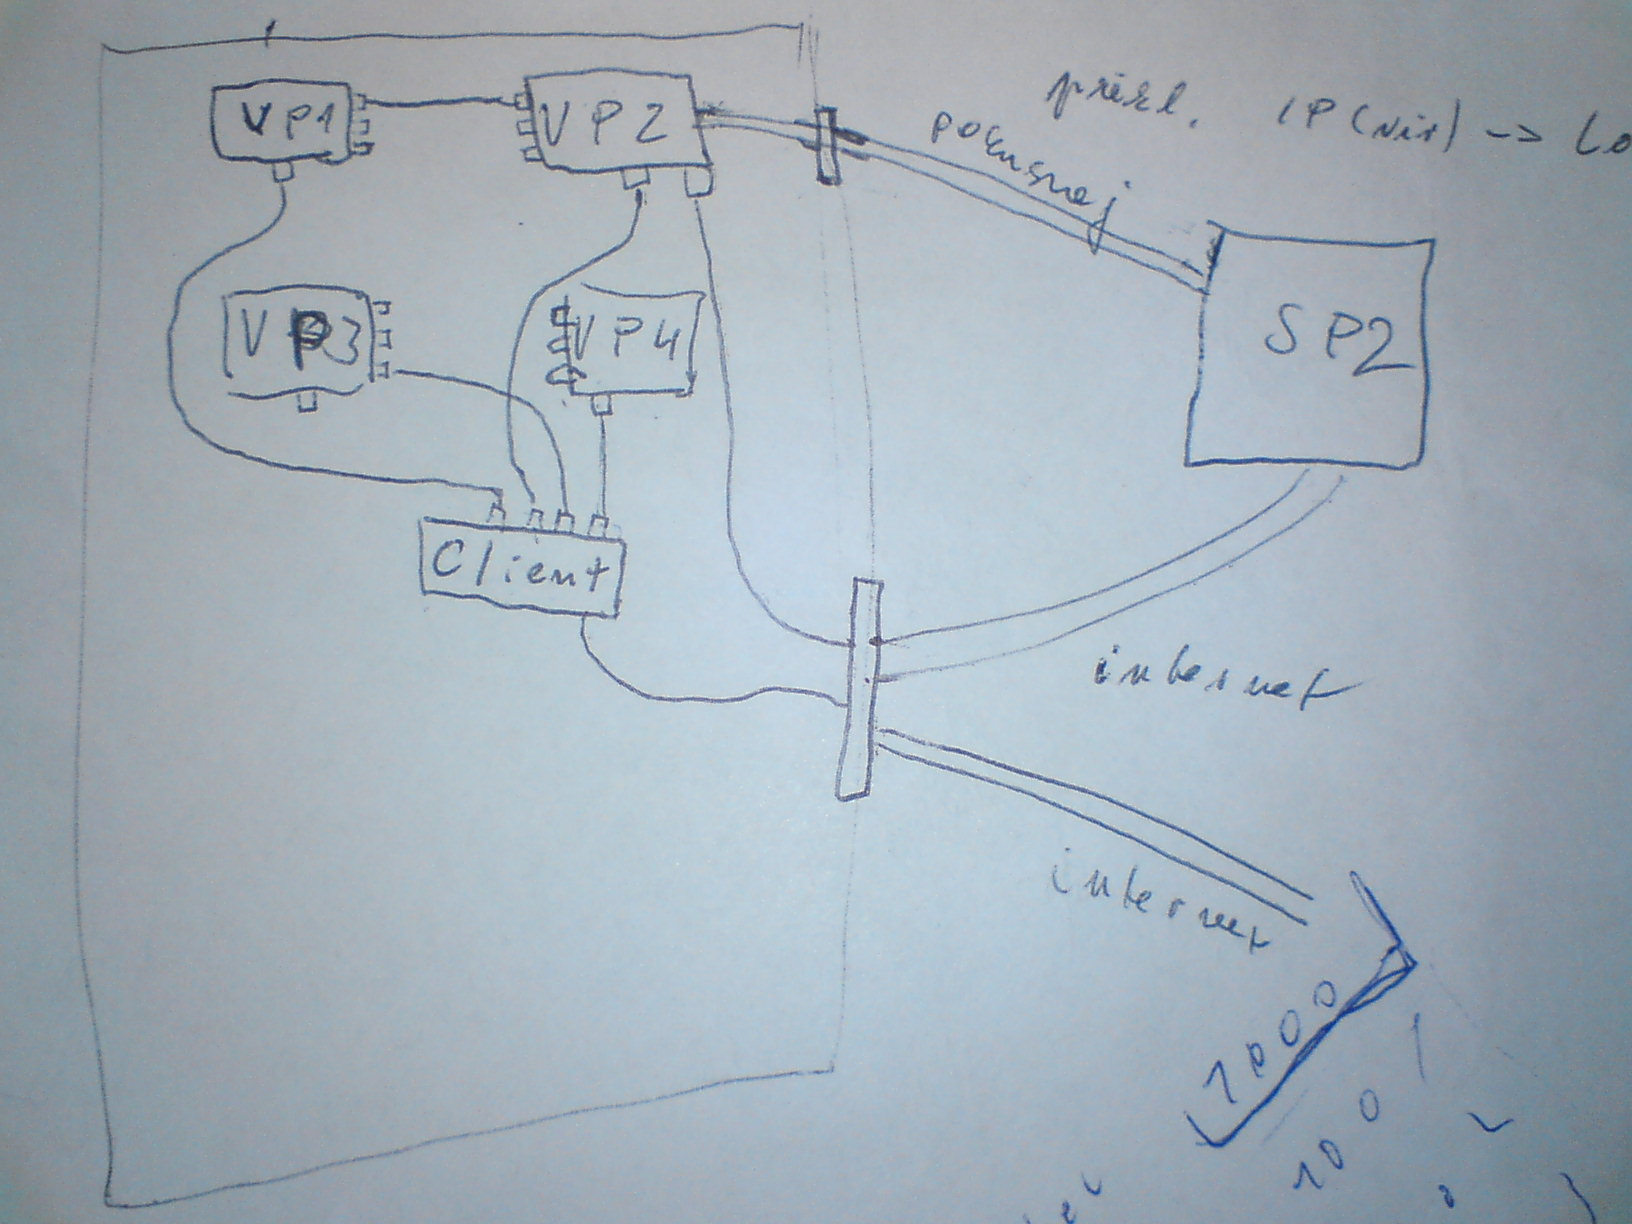
\includegraphics[width=9cm]{figures/navrh}
\caption{Počáteční návrh}
\label{fig:navrh}
\end{center}
\end{figure}

%------------------------------------------------------------------------------

\subsection{Klient - server}\label{klien_server}
Síťovou vrstvu systému tvoří architektura klient - server. Ta, jak jsem již naznačoval v kapitole \ref{vymezeni}, byla převzata ze semestrální práce, kde bylo za úkol mimo jiné implementovat více-vláknový server. Server má sám pro sebe vlastní vlákno ve kterém běží. Dále server vytvoří při startu pro všechny počítače nová vlákna, která poslouchají na portu o jedna větším než předchozí počítač (první počítač začíná na portu předaným jako parametr při startu serveru). Tyto vlákna se chovají zase jako servery. Když se uživatel připojí na libovolný počítač, tak se vytvoří další vlákno pro obsluhu tohoto klienta. Výhodou tohoto řešení je, že je možné se připojit na kterýkoliv počítač kolikrát potřebujeme. Je to tedy přesně tak, jako bychom se připojovali na reálné Cisco či Linux např. přes protokol ssh\footnote{Secure Shell - zabezpečený komunikační protokol (v současné době náhrada telnetu)} či telnet.

\begin{figure}[h]
\begin{center}
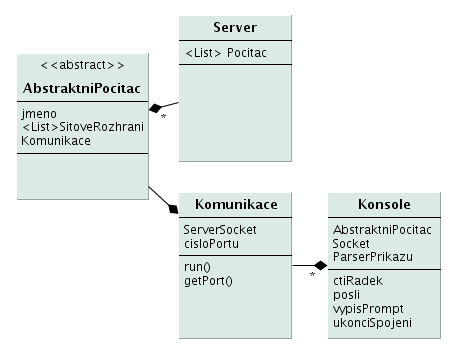
\includegraphics[width=9cm]{figures/uml_sit2}
\caption{Návrh komunikační části}
\label{uml:sit}
\end{center}
\end{figure}

Na obrázku \ref{uml:sit} je znázorněna komunikační část pomocí UML\footnote{Unified Modeling Language, UML je v softwarovém inženýrství grafický jazyk pro vizualizaci, specifikaci, navrhování a dokumentaci programových systémů.\cite{wiki:uml}} diagramu. Každý počítač má objekt \verb|Komunikace|, která čeká na připojení nového klienta. Když klient vyšle požadavek o nové spojení, tak se vytvoří \verb|Konsole|, která tohoto klienta bude obsluhovat. Při odpojení klienta \verb|Konsole| zaniká, protože její přítomnost už není potřeba.

%------------------------------------------------------------------------------

\subsection{Vyhodnocování příkazů}
Když uživatel zadá příkaz a ukončí ho znakem nového řádku (klávesa Enter, znak \verb|\n|), tak se ve třídě \verb|Konzole| zavolá metoda \verb|zpracujRadek()|. Tuto metodu vlastní abstraktní \verb|ParserPrikazu|, který je v mém případe implementován jako \verb|CiscoParserPrikazu|\footnote{LinuxParser příkazů má na starosti kolega. Pro jiné typy počítačů je nutno implementovat parser vlastní.}. Ten se stará o zpracování poslané řádky a podle toho volá různé Cisco příkazy, které tvoří můj IOS, či jiné servisní příkazy.

% \newpage

%------------------------------------------------------------------------------

\subsection{Datové struktury jádra}

Po architektuře klient - server bylo potřeba domyslet datové struktury virtuálních počítačů. Ze začátku jsem nastínil základní třídy a zbytek jsem dodělával jak bylo potřeba. 

\subsubsection{Směrovač - CiscoPocitac}
Na skutečné počítačové síti jsou síťové prvky několika druhů (switche, bridge, repeatery, směrovače, ..), ale na laboratorních cvičeních předmětu Y36PSI se  nastavují pouze směrovače ze 3. vrstvy\footnote{Tato \uv{síťová vrstva} se stará o směrování v síti a síťové adresování. Dále poskytuje spojení mezi vzdálenými sítěmi, které spolu přímo nesousedí.} síťového ISO/OSI modelu. Proto v mé práci figuruje pouze jeden typ síťového prvku - směrovač (router), který je reprezentován datovou strukturou \verb|CiscoPocitac| viz obrázek \ref{uml:class}. Ten je spojen přes vlastní rozhraní k jinému počítači přes jeho rozhraní právě jedním \uv{kabelem}. Není tedy možné, aby bylo jedno rozhraní připojeno k více rozhraním, protože jsou to všechno dvou bodové spoje. 

% \newpage

\begin{figure}[h]
\begin{center}
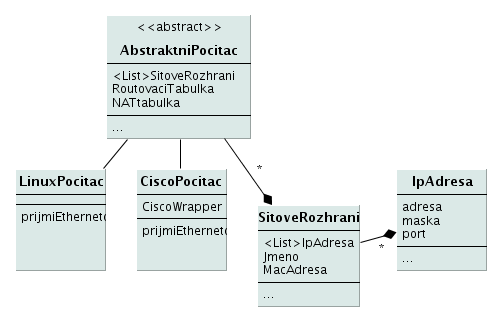
\includegraphics[width=10cm]{figures/uml_class}
\caption{Zjednodušený diagram tříd}
\label{uml:class}
\end{center}
\end{figure}

Nastavení propojení mezi počítači (respektive jejich rozhraními) je dáno v konfiguračním souboru. Původně každé rozhraní obsahovalo informaci, ke kterému rozhraní kterého počítače je připojeno. To se ale ukázalo jako zbytečně matoucí, protože informace o kabelu tam byla obsažena dvakrát. V dnešní verzi programu je to zjednodušené tak, že samotné rozhraní nenese žádnou informaci o kabelu. Ale kabely jsou konfiguračním souboru zvlášť:

\begin{verbatim}
<kabelaz>
  <kabel>
    <prvni>linux1:eth0</prvni>
    <druhy>linux2:eth0</druhy>
  </kabel>
  <kabel>
    <prvni>linux2:eth1</prvni>
    <druhy>cisco1:FastEthernet0/0</druhy>
  </kabel>
  <kabel>
    <prvni>cisco1:FastEthernet0/1</prvni>
    <druhy>cisco2:FastEthernet0/0</druhy>
  </kabel>
</kabelaz>
\end{verbatim} 

Konce kabelu jsou charakterizovány dvěma záznamy, každý obsahuje jméno počítače a rozhraní oddělené dvojtečkou.

% \newpage

\subsubsection{Síťové rozhraní}
Datová struktura pro síťové rozhraní je ve své podstatě jednoduchá. Obsahuje jméno, seznam IP adres přiřazených k tomuto rozhraní, MAC\footnote{MAC - Media Access Control, je fyzická adresa, kterou používá 2. (spojová) vrstva ISO/OSI modelu} adresu a stav.

Systémem je oficiálně podporována pouze jedna IP adresa per rozhraní, více adres si ale vyžádal překlad adres. MAC adresa je v tomto systému spíše pro větší přiblížení skutečnému rozhraní, protože ARP\footnote{\uv{Address Resolution Protocol se v počítačových sítích s IP protokolem používá k získání ethernetové MAC adresy sousedního stroje z jeho IP adresy. Používá se v situaci, kdy je třeba odeslat IP datagram na adresu ležící ve stejné podsíti jako odesilatel. Data se tedy mají poslat přímo adresátovi, u něhož však odesilatel zná pouze IP adresu. Pro odeslání prostřednictvím např. Ethernetu ale potřebuje znát cílovou ethernetovou adresu.}\cite{wiki:arp}} protokol není u nás přímo implementován. Systém obsahuje pouze několik pravidel, které byly nutné pro rozhodování zda přijmout či nepřijmout příchozí paket. Dále rozhraní obsahuje indikátor stavu, ve kterém se nachází - zapnuté/vypnuté. Tento ukazatel jsem zavedl, protože rozhraní Cisca jsou ve výchozím stavu vypnutá.

\subsubsection{IP adresa}
IP adresa je mnohem složitější než rozhraní i když obsahuje pouze tři čísla reprezentující adresu, masku a port. Složitost je dána tím, že tato třída obsahuje přes 40 obslužných metod, které pokrývají veškerou práci, co je potřeba s adresou dělat.

%------------------------------------------------------------------------------

\subsection{Telnet}
V zadání je přímo zmíněno použití programu telnet pro připojení klientů k serveru. Telnet je ale také protokol, po kterém se domlouvá telnet klient a telnet server. Česká wikipedie píše o telnet protokolu: \uv{Protokol přenáší osmibitové znaky oběma směry (duplexní spojení) a je velmi jednoduchý.\cite{wiki:telnet}}. Podle protokolu se vše posílá po znaku a protistrana po znaku vše potvrzuje. Protokol telnet ale zas tak jednoduchý není. Podporuje několik režimů, při navazování spojení začne proces vyjednávání atd. To všechno implementovat by bylo na samostatnou (možná i diplomovou) práci. 

Samotný telnet (ať protokol či program) ale neposkytuje doplňování příkazů nebo alespoň historii příkazů. Dalším problémem je, že při psaní příkazů přes telnet nefunguje editace aktuálního řádku, respektive lze mazat po znacích klávesou \verb|BackSpace|, ale nelze se pohybovat do stran šipkami doleva a doprava - při takovém pokusu to vypíše \verb|^[[D| či \verb|^[[C|. Tato \uv{vlastnost} se ale neprojevuje při připojování na vlastní telnet server. To je způsobeno tím, že v takovém případě se o editaci řádku a historii příkazů stará samotný BASH\footnote{Bourne again shell - nejpoužívanější unixový shell}. V případě této aplikace toho ale nelze využít, tak jsem se rozhodl, že tyto funkcionality budou na straně klienta, kde to bude zajišťovat \uv{někdo jiný}. 

Pro Linux jsem našel program rlwrap (readline wrapper), který přidává všechny tyto užitečné funkce: editace řádky, historie příkazů, doplňování příkazů, obarvení promptu. Pro Windows jsem nic takového nenašel, takže je to vyřešeno tak, že se vše pouští pod programem Cygwin. Navíc toto řešení zvyšuje komfort práce pod Windows, jelikož program \verb|cmd| není úplně uživatelsky přívětivý.

%------------------------------------------------------------------------------

\section{Podobnost simulátoru se skutečným Ciscem}\label{kap:podobnost}
Při implementaci jsem se snažil vytvořit systém, který bude co nejvíce podobný skutečnému Ciscu. Musel jsem ale někde položit hranici mezi složitostí a věrností výsledné práce, protože tyto dvě metriky jsou vzájemném protikladu. Cisco IOS je natolik robustní a propracovaný systém, že je v mých silách pouze implementace úzké části systému, která je nutně potřeba pro splnění cíle. Byl jsem přinucen místy ustoupit a nechat vypsat hlášení, že to či ono není podporováno. V samotném parseru příkazů není toto téměř vůbec řešeno, protože by to znamenalo dopsání dohromady několika stovek pravidel pro všechny příkazy - např. příkaz \verb|ip| má 103 možností v konfiguračním stavu. Aby ale uživatel měl alespoň nějakou možnost se dopátrat, co je podporováno a co ne, tak jsem přidal příkaz \verb|help| (\verb|help_en| pro výpis v angličtině), který popisuje, co lze v jakém stavu Cisca použít.

%------------------------------------------------------------------------------

\section{Programovací jazyk a prostředí}
Pro implementaci simulátoru jsem si vybral programovací jazyk Java hned z několika důvodů. Jazyk je to velmi robustní s bohatou sadou různých knihoven. Navíc programy vytvořené v tomto jazyce jsou zpravidla jednoduše přenositelné mezi různými operačními systémy, což je jeden z bodů nefunkčních požadavků. Jazyk Java disponuje propracovaným systémem výjimek, takže při nějaké neočekávané chybě se dozvíme víc, než v jazyce C++ s jeho \verb|Segmentation fault|. Neméně významným důvodem je i skutečnost, že s Javou mám zatím největší zkušenosti.

Celou práci jsem implementoval v Netbeans IDE\footnote{Integrated Development Environment} verze 6.8.

%------------------------------------------------------------------------------

\section{Uživatelské rozhraní}
Uživatelské rozhraní je v zásadě velmi jednoduché. Vše je ovládáno přes příkazovou řádku, tak jak jsme zvyklí. Spuštění serveru je ulehčeno pomocným skriptem \verb|start_server.sh|, který zároveň obsahuje nápovědu. Pro připojování klientů jsem připravil skripty, ve kterých je zohledněna verze programu rlwrap. V balíčku programu Cygwin je rlwrap starší verze, která neumožňuje obarvování promptu a přeposílání signálů (např. při zmáčknutí Ctrl+C nebo Ctrl+Z). Novější verze už tyto funkce mají. Skripty pro připojení na \verb|linux.sh| a \verb|cisco.sh| fungují nezávisle na verzi.

\begin{figure}[h]
\begin{center}
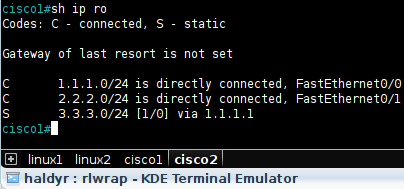
\includegraphics[height=2.5cm]{figures/uziv_rozhrani}
\caption{Uživatelské rozhraní pod OS Linux}
\label{fig:uziv_rozh}
\end{center}
\end{figure}

%------------------------------------------------------------------------------

\section{Skutečné Cisco}
Jedním z největších \uv{oříšků} této práce bylo zjistit, jak se chová skutečné Cisco. Pravdou je, že Cisco Systems má na svých stránkách slušnou řadu návodů, nicméně není tak jednoduché v nich najít, co zrovna potřebujeme. A tak jsem hodně věcí zjišťoval z živého Cisca umístěného na Karlově náměstí přes protokol ssh. 








